\begin{enumerate}
	\item L'utilisateur clique sur son nom dans la bar de navigation.
	\item L'utilisateur clique sur \textit{Profil} dans le menu déroulant.
	\item L'utilisateur retrouve l'information dans le cadre afficher sur la page.
\end{enumerate}

\newpage
\begin{figure}[h]
	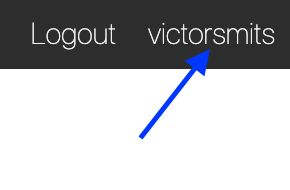
\includegraphics[width=0.5\textwidth,center]{Figures/us7-1}
	\caption{Bouton de navigation vers le profil}
\end{figure}

\vspace{\baselineskip}
\begin{figure}[h]
	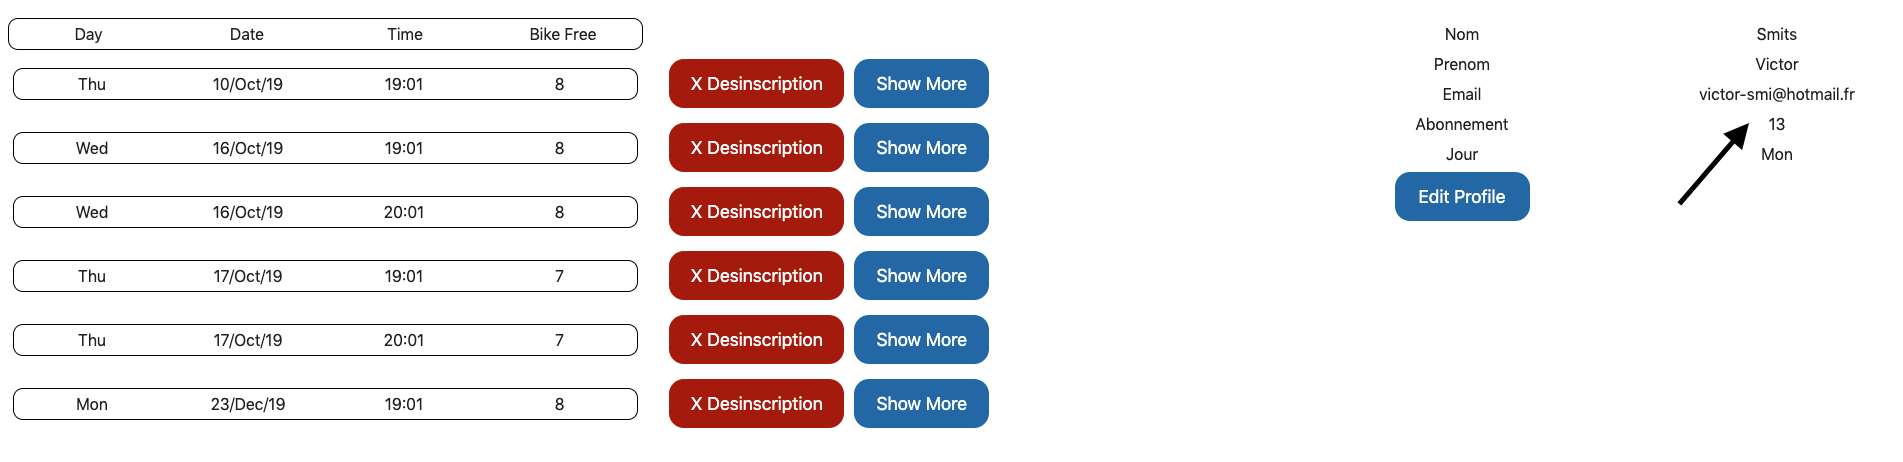
\includegraphics[width=0.5\textwidth,center]{Figures/us7-2}
	\caption{Nombre de séance restante dans l'abonnement}
\end{figure}

